\section{ManiGit Architecture}
\label{sec:manigit_architecture}

ManiGit is designed as a modular, transparent infrastructure layer situated between the raw conversational dialogue stream and the LLM inference runtime. Fig.~\ref{fig:architecture} illustrates the overall system architecture, and Fig.~\ref{fig:memory_lifecycle} details the memory lifecycle state machine.

\begin{figure*}[t]
\centering
\resizebox{0.95\textwidth}{!}{%
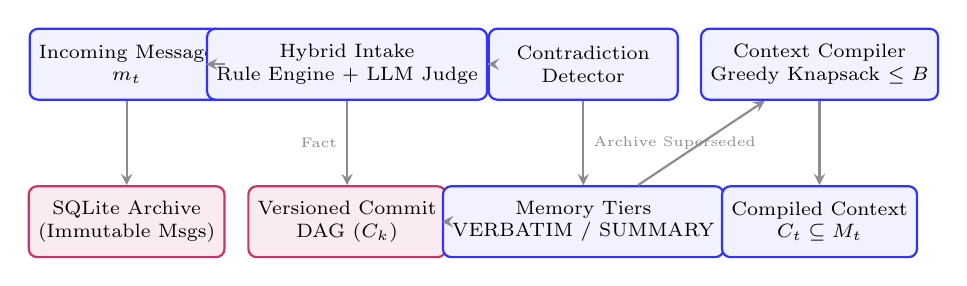
\begin{tikzpicture}[
    box/.style={rectangle, draw=blue!80, fill=blue!5, thick, rounded corners=3pt, minimum width=2.4cm, minimum height=0.9cm, align=center, font=\scriptsize},
    databox/.style={rectangle, draw=purple!80, fill=purple!8, thick, rounded corners=3pt, minimum width=2.4cm, minimum height=0.9cm, align=center, font=\scriptsize},
    flow/.style={->, >=stealth, thick, color=gray!90}]

\node[box] (msg) {Incoming Message\\$m_t$};
\node[box, right of=msg, xshift=1.8cm] (class) {Hybrid Intake\\Rule Engine + LLM Judge};
\node[databox, below of=msg, yshift=-1.0cm] (rawdb) {SQLite Archive\\(Immutable Msgs)};
\node[databox, right of=rawdb, xshift=1.8cm] (dag) {Versioned Commit\\DAG ($C_k$)};
\node[box, right of=class, xshift=2.0cm] (contra) {Contradiction\\Detector};
\node[box, right of=dag, xshift=2.0cm] (tiers) {Memory Tiers\\VERBATIM / SUMMARY};
\node[box, right of=contra, xshift=2.0cm] (compiler) {Context Compiler\\Greedy Knapsack $\le B$};
\node[box, below of=compiler, yshift=-1.0cm] (prompt) {Compiled Context\\$C_t \subseteq M_t$};

\draw[flow] (msg) -- (class);
\draw[flow] (msg) -- (rawdb);
\draw[flow] (class) -- node[left, font=\tiny]{Fact} (dag);
\draw[flow] (class) -- (contra);
\draw[flow] (contra) -- node[right, font=\tiny]{Archive Superseded} (tiers);
\draw[flow] (dag) -- (tiers);
\draw[flow] (tiers) -- (compiler);
\draw[flow] (compiler) -- (prompt);

\end{tikzpicture}%
}

\caption{ManiGit system architecture: Raw messages are stored immutably in SQLite. The hybrid intake pipeline classifies candidate facts into functional tiers and commits them to the versioned DAG. The contradiction detector identifies superseding facts, archiving older versions and recording Why Reports. The context compiler executes a greedy knapsack selection over active memories to assemble a budget-constrained context window $C_t \le B$ for the model adapter.}
\label{fig:architecture}
\end{figure*}

\begin{figure}[t]
\centering
\resizebox{0.92\columnwidth}{!}{%
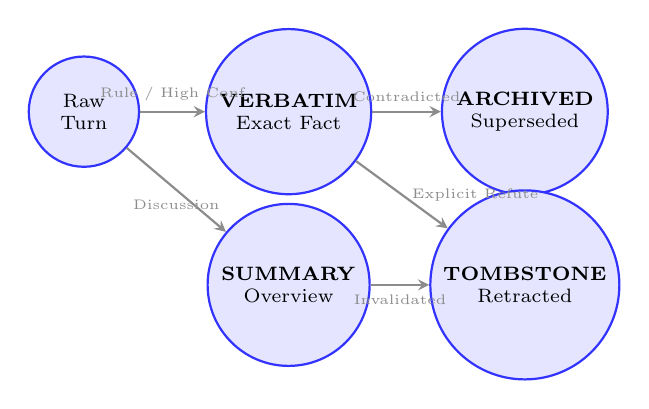
\begin{tikzpicture}[
    state/.style={circle, draw=blue!80, fill=blue!10, thick, minimum size=1.4cm, align=center, font=\scriptsize},
    trans/.style={->, >=stealth, thick, color=gray!90}]

\node[state] (raw) {Raw\\Turn};
\node[state, right of=raw, xshift=1.6cm] (verb) {\textbf{VERBATIM}\\Exact Fact};
\node[state, below of=verb, yshift=-1.2cm] (summ) {\textbf{SUMMARY}\\Overview};
\node[state, right of=verb, xshift=2.0cm] (arch) {\textbf{ARCHIVED}\\Superseded};
\node[state, right of=summ, xshift=2.0cm] (tomb) {\textbf{TOMBSTONE}\\Retracted};

\draw[trans] (raw) -- node[above, font=\tiny]{Rule / High Conf} (verb);
\draw[trans] (raw) -- node[below, font=\tiny]{Discussion} (summ);
\draw[trans] (verb) -- node[above, font=\tiny]{Contradicted} (arch);
\draw[trans] (summ) -- node[below, font=\tiny]{Invalidated} (tomb);
\draw[trans] (verb) -- node[right, font=\tiny]{Explicit Refute} (tomb);

\end{tikzpicture}%
}

\caption{ManiGit four-tier memory lifecycle state machine. Raw dialogue turns transition into \texttt{VERBATIM} (exact constraints/decisions) or \texttt{SUMMARY} (high-level overviews). When contradicted, facts transition to \texttt{ARCHIVED}; explicit refutations transition facts to \texttt{TOMBSTONE}.}
\label{fig:memory_lifecycle}
\end{figure}

\subsection{Immutable Message Archive}
All incoming raw messages $m_t$ (from both user and assistant turns) are appended directly to an immutable SQLite repository. Each record stores:
$$\text{Record}(m_t) = \langle \text{id}, \text{session\_id}, \text{role}, \text{content}, \text{timestamp}, \text{content\_hash} \rangle$$
where $\text{content\_hash}$ is computed via SHA-256 over normalized message content. Messages cannot be mutated or deleted under any circumstance, establishing an immutable, content-addressed ground truth.

\subsection{Hybrid Rule-First Memory Classification}
Raw conversational turns contain a mixture of casual dialogue, transient pleasantries, and critical technical instructions. Storing every turn as a memory fact causes memory bloat; conversely, running an LLM on every turn introduces severe latency.

ManiGit implements a two-stage hybrid intake pipeline:
\begin{enumerate}
    \item \textbf{Rule Engine (Stage 1):} Evaluates incoming turns against deterministic regex pattern rules targeting high-priority signals (explicit constraints, database selections, credentials, API endpoints). If a rule matches, the fact is immediately classified into the \texttt{VERBATIM} tier with maximum confidence ($c = 1.0$) and zero API latency.
    \item \textbf{LLM Judge (Stage 2):} Turns not matching deterministic rules fall through to an LLM judge calibrated with explicit confidence thresholds:
    $$\text{Tier}(f) = \begin{cases}
    \texttt{VERBATIM}, & \text{if } c \ge 0.85 \text{ and is\_constraint}(f) \\
    \texttt{SUMMARY},  & \text{if } c \ge 0.70 \text{ and is\_discussion}(f) \\
    \texttt{ARCHIVED}, & \text{if } c < 0.70 \text{ (speculative / uncertain)}
    \end{cases}$$
\end{enumerate}

\subsection{Versioned Commit DAG}
Instead of updating memory records in place, ManiGit models memory states as commits in a Directed Acyclic Graph (DAG). A commit $C_k$ encapsulates:
$$C_k = \langle \text{commit\_hash}, \text{parent\_hash}, \text{branch}, \text{message}, \text{timestamp}, \mathcal{M}_k \rangle$$
where $\mathcal{M}_k = \{m_1, m_2, \dots, m_n\}$ denotes the set of active memory objects valid at that commit. Commits are linked via SHA-256 parent hashes, exactly mirroring Git repository semantics. Branch isolation enables agents to explore alternative reasoning branches without contaminating the production memory branch.

\subsection{Bidirectional Provenance & Why Reports}
Every memory object $m_i \in \mathcal{M}_k$ maintains explicit bidirectional provenance:
\begin{itemize}
    \item \textbf{Source Linkage:} Pointers to the originating message ID ($\text{source\_msg\_id}$) and turn index.
    \item \textbf{Why Report:} A structured audit document recording:
    $$\text{WhyReport}(m_i) = \langle \text{rule\_id}, \text{judge\_confidence}, \text{decision\_rationale}, \text{superseded\_target\_id} \rangle$$
\end{itemize}
This ensures that any memory accessed during context compilation can be directly traced back to its originating conversation turn and classification rationale via explicit relational provenance links.

\subsection{Automated Contradiction Detection & Supersession}
When a new memory fact $m_{\text{new}}$ is classified, ManiGit executes semantic conflict detection against all active memories in the current branch. If $m_{\text{new}}$ supersedes or contradicts an active fact $m_{\text{old}}$:
\begin{enumerate}
    \item $m_{\text{old}}$ is transitioned from its current tier to \texttt{ARCHIVED}.
    \item The supersession relationship is recorded in $m_{\text{new}}$'s Why Report ($\text{supersedes} = m_{\text{old}}.\text{id}$).
    \item A new commit $C_{k+1}$ is generated where $\mathcal{M}_{k+1} = (\mathcal{M}_k \setminus \{m_{\text{old}}\}) \cup \{m_{\text{new}}\}$.
\end{enumerate}
Because $m_{\text{old}}$ is archived rather than deleted, it is completely removed from subsequent prompt context compilation, preventing ghost context while remaining fully recoverable in historical commit states.

\subsection{Context Compilation under Token Budgets}
When the agent receives a user query $q_t$, the Context Compiler dynamically selects a subset of active memories $C_t \subseteq \mathcal{M}_k$ that maximizes relevance while strictly adhering to a pre-allocated token budget $B$. The formal mathematical optimization and greedy knapsack compilation are detailed in Section~\ref{sec:mathematical_formulation}.

\subsection{Point-in-Time Historical Reconstruction}
ManiGit supports deterministic time travel. By invoking:
$$\text{checkout}(C_{\text{target}})$$
the Context Compiler reconstructs the exact active memory set $\mathcal{M}_{\text{target}}$ as it existed at commit $C_{\text{target}}$ and compiles a budget-compliant context window for that past moment. This enables agents to answer historical retrospective questions deterministically without polluting current branch state, achieving 100\% point-in-time reconstruction across evaluated benchmark scenarios.
